\tikzstyle{bloc3} = [rectangle, rounded corners, minimum width=3.5cm, minimum height=2.5cm, text centered, fill=white, align=center]
\tikzstyle{inout} = [anchor=south, align=center, node distance=1.5cm]
\begin{tikzpicture}[node distance=4.25cm]
    \node (cntloc_u) [bloc3] {
        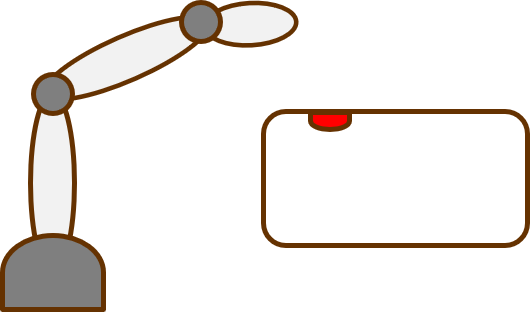
\includegraphics[width=0.10\textwidth]{images/ptraj_1.png} \\
        \small{Location} $p_u^t$ on \small{the object} 
        };
    \node (cntloc_a) [bloc3, below of=cntloc_u, node distance=2.1cm] 
        {
        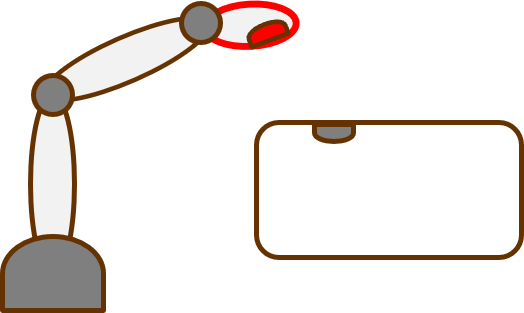
\includegraphics[width=0.10\textwidth]{images/ptraj_2.png} \\
        \small{Location} $p_a^t$ \small{on a link} $n_a$ 
        };
    \node (qstate_u) [bloc3, right of=cntloc_u] {
        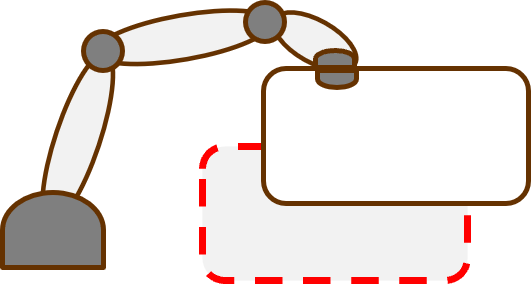
\includegraphics[width=0.10\textwidth]{images/ptraj_3.png} \\ 
        \small{Object pose} $q_u^t$ 
        };
    \node (qstate_a) [bloc3, below of=qstate_u, node distance=2.1cm] 
        {
        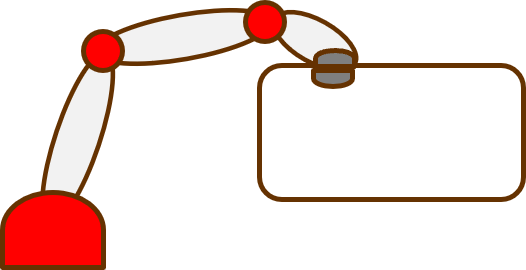
\includegraphics[width=0.10\textwidth]{images/ptraj_4.png} \\ 
        \small{Joint angles} $q_a^t$ 
        };
    \node (ucontr_u) [bloc3, right of=qstate_u] {
        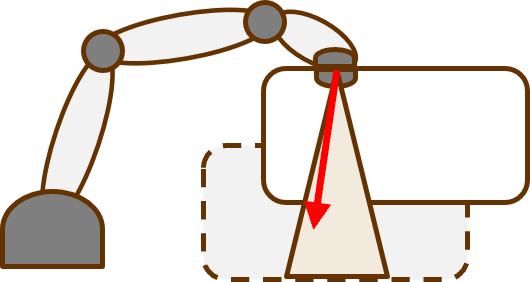
\includegraphics[width=0.10\textwidth]{images/ptraj_5.png} \\ 
        \small{Contact impulse} $\lambda_u^t$ 
        };
    \node (ucontr_a) [bloc3, below of=ucontr_u, node distance=2.1cm] 
        {
        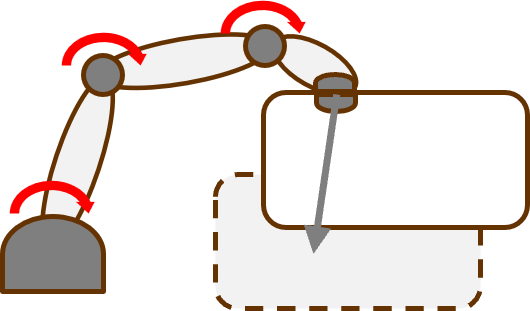
\includegraphics[width=0.10\textwidth]{images/ptraj_6.png} \\ 
        \small{Torque command} $\tau_a^t$ 
        };
    \node (col1) [inout, above of=cntloc_u, node distance=1.2cm]  {\textbf{Contact location}};
    \node (col2) [inout, above of=qstate_u, node distance=1.2cm]  {\textbf{Configuration}};
    \node (col3) [inout, above of=ucontr_u, node distance=1.2cm]  {\textbf{Force/Torque}};
    % Vertical lines
    \draw ( 2.125, 1.5) -- (2.125,-2.9);
    \draw ( 6.375, 1.5) -- (6.375,-2.9);
    % Horizontal lines
    \draw (-1.7, 0.9) -- (10, 0.9);
    \draw (-1.7,-1.0) -- (10,-1.0);
\end{tikzpicture}
